

\chapter{PHILLIPO}

PHILLIPO é um \emph{solver} para campos de deformação elástica em estruturas discretizadas por elementos finitos, e segue a simbologia e o padrão dos algoritmos descritos por Zienkiewicz em sua obra intitulada \emph{The Finite Element Method}, com algumas otimizações computacionais relacionadas a paralelismo e matrizes esparsas, e que visa constituir-se como referência didática na implementação legível e concisa dos algoritmos de elementos finitos em Julia no âmbito acadêmico do campus CCT, da UDESC. PHILLIPO é um programa de código aberto, que é distribuído em um repositório público\footnotemark[1]{} sob a licença LGPL\footnotemark[2]{}. Portanto, sua utilização é gratuita e livre para fins acadêmicos e comerciais, que incluem a modificação, implementação e venda de qualquer parte do programa, como também da documentação que o acompanha; só se resguarda, entretanto, a devida citação deste documento.
\footnotetext[1]{O repositório é mantido no GitHub, assim como o presente documento em formato Latex: \url{https://github.com/lucas-bublitz/PHILLIPO}}
\footnotetext[2]{O GiD, interface de pré e pós-processamento, é um software distribuído comercialmente, e não está sujeito à mesma licença que PHILLIPO.}

PHILLIPO foi idealizado, a princípio, como um projeto de aplicação do método de elementos finitos em um contexto de programação estruturada, porém, observou-se que essa abordagem é, senão obsoleta, já muito utilizada em pesquisas científicas. Portanto, optou-se em trazer uma visão de projeto de software, alterando o paradigma para a programação em despachos múltiplos (um forma alternativa à orientação a objetos), uma vez que tópicos envolvendo esses assuntos não são muito discutidos nas cadeiras dos cursos de engenharia (menos a de software, é claro), e que as vantagens desse tipo de abordagem vão desde a legibilidade do código, até o reaproveitamento de estruturas de dados e funções.

Um \emph{solver}, ou em melhor português, um solucionador em MEF não é uma novidade no mundo acadêmico, nem no comercial. Softwares como Calculix (que é distribuído integrado com o FreeCAD) e o FreeFEM, que já conta com 7 mil commits em seu repositório, são continuamente produzidos e aprimorados desde antes da virada do milênio, um trabalho que demanda tempo e uma comunidade bem ativa.

Destarte, a pretensão de PHILLIPO não é fornecer uma alternativa a esses softwares, muito menos servir de módulo ou biblioteca para agregar algum deles, além do mais, a elaboração de programas robustos e confiáveis é um trabalho demorado e de muitas pessoas. O próprio FreeFEM já conta com mais de 7 mil commits em seu repositório, com a participação de 41 desenvolvedores. A pretenção de PHILLIPO é construir uma aplicação simples utilizando o MEF que possa aproveitar algumas ferramentas de contrução de código em Julia, como paralelismo e despachos múltiplos, para apresentar mais uma referência de programação em engenharia n
\section{O Projeto}

PHILLIPO foi idealizado para ser modular, implicando em ser encapsulado no sentido de que cada parte do código ao mesmo tempo que fosse integrada com o restante, fosse suficientemente independente a ponto de ser reutilizada por novas adições ao programa. Por conta disso, a elaboração de um conjunto de módulos e tipos, dentro do paradigma de despachos múltiplos, foi vital para alcançar essa meta, que não visa só a organização do código, mas sim, construir uma base forte o baste para possibilitar a fácil implementação futura de novas funcionalidades.

\section{Fluxo de execução}

O fluxo de execução é uma ferramenta de projeto que tem como objetivo descrever a ordem e as condições que determinadas seções do código são executadas. A utilização de PHILLIPO.jl segue os digramas das figuras \ref{fig:fluxograma_GID} e \ref{fig:fluxograma_PHILLIPO}

\begin{figure}
    \centering
    \caption{Fluxograma de execução: GID}
    \includegraphics[width = \textwidth]{Figuras/fluxograma_GID.pdf}
    \label{fig:fluxograma_GID}
\end{figure}

\begin{figure}
    \centering
    \caption{Fluxograma de execução: PHILLIPO.jl}
    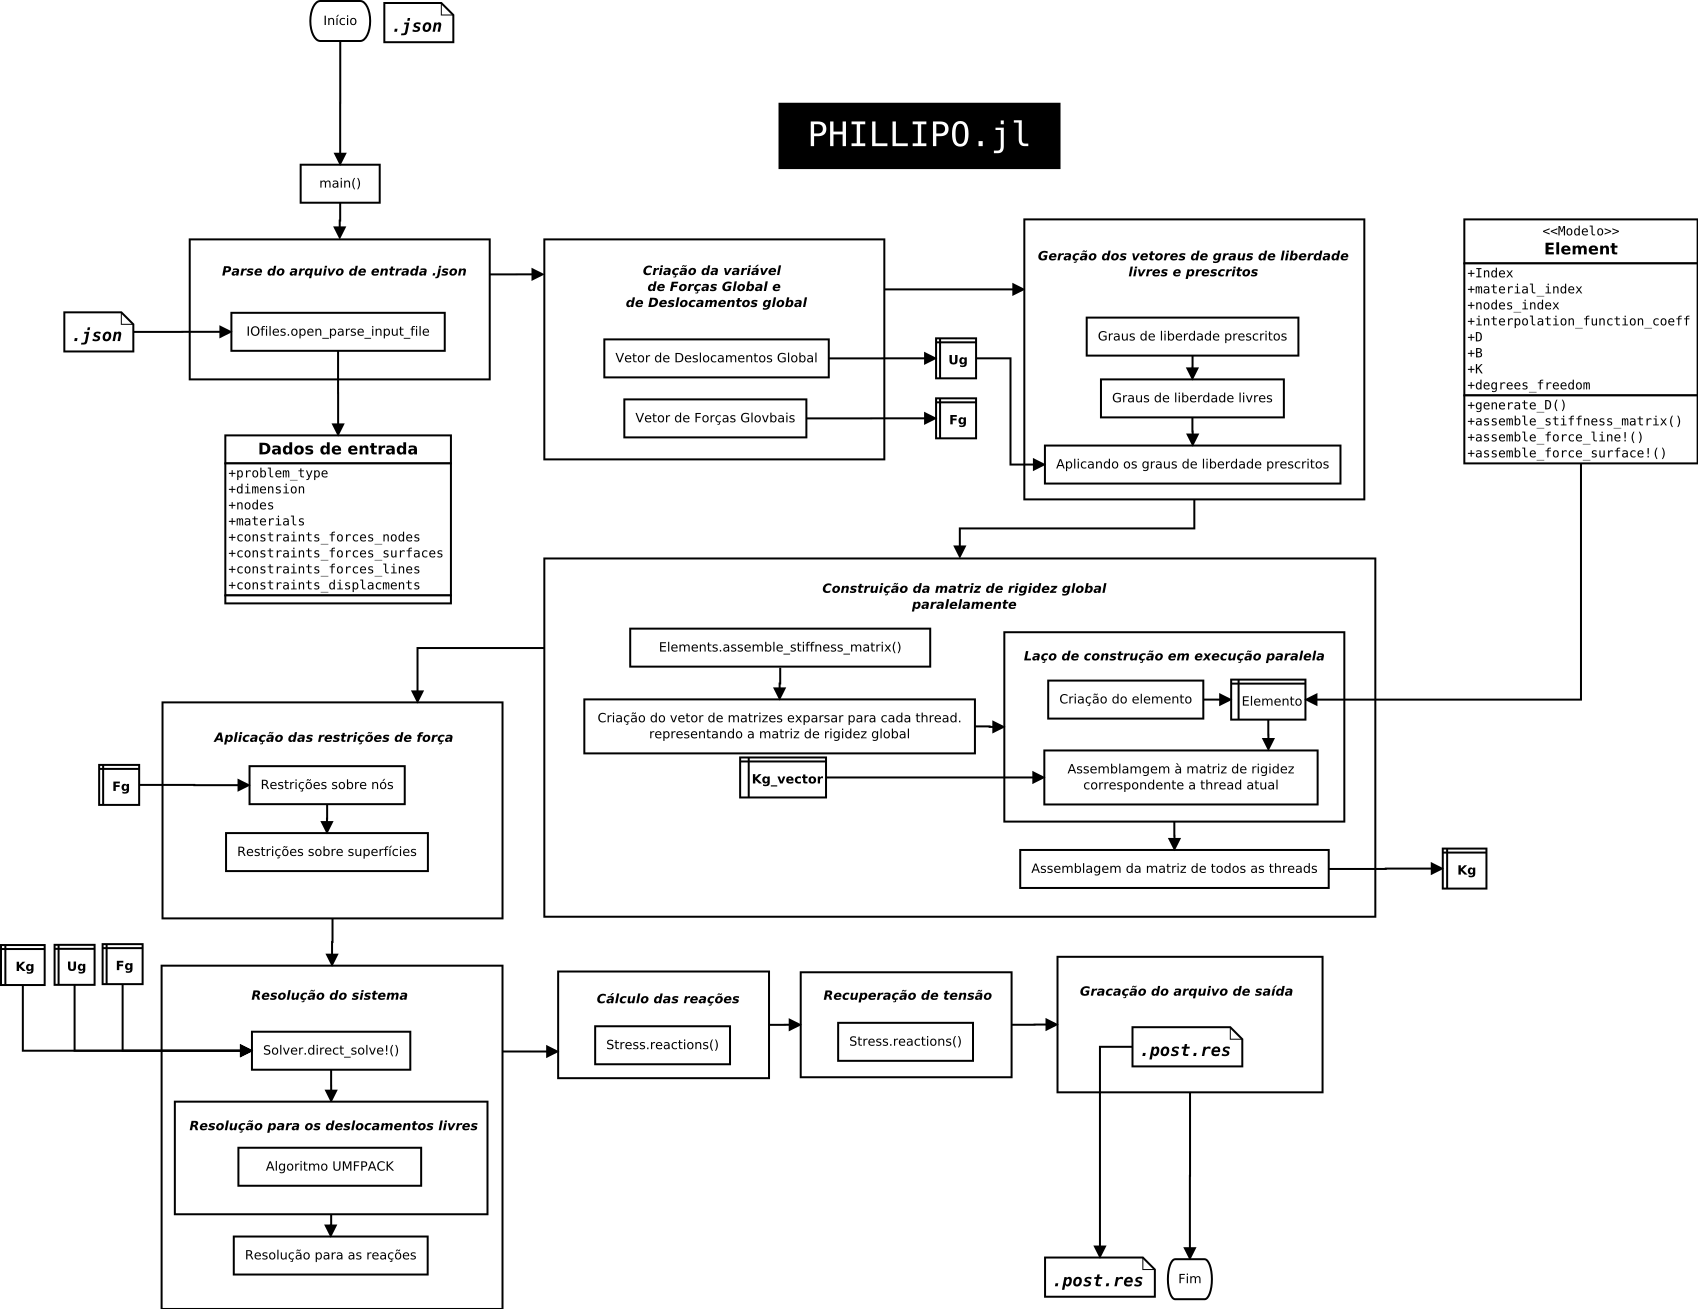
\includegraphics[width = \textwidth]{Figuras/fluxograma_PHILLIPO.pdf}
    \label{fig:fluxograma_PHILLIPO}
\end{figure}